\documentclass[en]{../../../../../../eplexam}
\usepackage{../../../../../../eplunits}
\usepackage{circuitikz}
\usepackage{pgfplots}
\pgfplotsset{compat=newest}

\hypertitle{circmes-ELEC1370}{4}{ELEC}{1370}{2016}{Juin}
{Nicolas Verbeek\and Adrien Couplet\and Martin Van Essche\and Guillaume Gilson\and Guillaume Colinet}
{Claude Oestges, Bruno Dehez and Christophe Craeye}

\section{Question Oestges : phaseurs}
Soit le circuit ci-dessus, avec $I_o = 10\angle\ang{350}$.
\begin{center}
	\begin{circuitikz} \draw
		to[european resistor,l=$Z_\alpha$, i_>=$I_x$, -*] (0,2.5) to[american current source,l=$2\angle 0^\circ$A] (2.5,2.5)
 		(2.5,0) to[american voltage source, l=$12\angle 0^\circ$V,-*] (2.5,2.5)
 		(2.5,2.5) to[R, l=$\SI{1}{\ohm}$] (5,2.5)
  		to[R,l=$\SI{1}{\ohm}$, i_>=$I_o$,*-] (5,0)
 		(0,0) -- (5,0)
 		(0,2.5) to[R,l=$\SI{1}{\ohm}$] (0,5) -- (2.5,5) to[L,l=$j\SI{1}{\ohm}$,*-] (2.5,2.5)
 		(2.5,5) -- (5,5) to[C,l=$-j\SI{1}{\ohm}$] (5,2.5);
	\end{circuitikz}
\end{center}
On demande:
\begin{enumerate}
    \item Le courant $I_x$
    \item L'impédance $Z_\alpha$
    \item La tension dans la source de courant
    \item La puissance de la source de tension
\end{enumerate}
\begin{solution}
Solutions finales (contrôlées avec LTSpice):
\begin{enumerate}
    \item $I_x = 2.17\angle 83.02^\circ$ A
    \item $Z_\alpha = 3.98\angle 39.5^\circ \Omega$
    \item $V_s = 10.35\angle 44.67^\circ$ V
    \item $P = -\SI{57.48}{\watt}$
\end{enumerate}
\end{solution}

\section{Question Oestges : Bode et quadripôles} 
Soit le circuit avec amplificateurs opérationnels idéaux
\begin{center}
    \begin{circuitikz}[scale = 0.9, transform shape]
		\draw
		(-1,1) node [above]{$V_\text{in}$} to [short,o-] (-0.5,1) 
		to [R, l=$R_1$] (2,1)
		(6,0.5) node[op amp] (opamp) {}
		(opamp.-) to [C,-*,l_=$C$] (2,1) 
		(opamp.+) to [short] (4,0)
		(opamp.out) to [short] (8,0.5)
		(4.5,1) to [short,*-] (4.5,2.5) to [R,l=$R_2$,-*] (8,2.5)
		(4,0) -- (4,-0.5) node [ground] {}
		(2,1) -- (2,4) to [C,l=$C$] (8,4) to [short,-*] (8,0.5) to [R,l=$R_3$,-*] (11,0.5) -- (12,0.5)
		(-0.5,1) to [short,*-] (-0.5,-2) to [R,l=$R$] (11,-2) -- (11,0.5)

		(14,0) node[op amp] (opamp2) {}
		(opamp2.-) to [short,-*] (12,0.5) 
		(opamp2.+) to [short] (12,-0.5)
		(12,-0.5) -- (12,-1) node [ground] {}
		(opamp2.out) to [short,-*] (15.5,0)

		(12,0.5) -- (12,2) to [R, l=$R$] (15.5,2) -- (15.5,0) to [short,-o] (16,0) node [above]{$V_\text{out}$};
	\end{circuitikz}
\end{center}

On demande:
\begin{enumerate}
    \item La fonction de transfert $\frac{V_\text{out}}{V_\text{in}}$
    \item Le diagramme de Bode de la fonction de transfert trouvée au point précédent
    \item L'impédance de sortie $Z_\text{out}$ en sachant que $Z_\text{in}=\SI{50}{\ohm}$
\end{enumerate}
En vous aidant des données numériques suivantes : $R_1 = \SI{21.6}{\kilo\ohm}$, $R_2 = \SI{28.8}{\kilo\ohm}$, $R_3 = \SI{10}{\kilo\ohm}$, $R = \SI{30}{\kilo\ohm}$, $C = \SI{1}{\nano\farad}$
\nosolution

\section{Question Dehez : pont de Wheatstone} 
Soit le pont de Wheatstone un peu modifié. 
\begin{center}
    \begin{circuitikz}[european resistors]
        \def\x{6}
        \def\y{6}
        % Size of the bridge
        \def\dx{3}
        \def\dy{3}
        % Voltage source
        \draw (0,0) to [sinusoidal voltage source, l=$V_s\; \omega_0$]
        (0, \y) to (\x, \y)
        % Left half bridge
        to [american resistor, l_=$R$, *-*] (\x-\dx,\y-\dy) % Top left resistor
        to [vR, l_=$Z_m$, -*] (\x,\y-2*\dy);  % Bottom left resistor
        % Right half bridge
        \draw (\x,\y)
        to [american resistor, l=$R_x$] (7.5, 4.5) % Top right resistor
        to [L, l=$L_x$,-*] (\x+\dx, \y-\dy)
        to [american resistor, l_=$R$, -*] (\x,\y-2*\dy)  % Bottom right resistor
        % Draw connection to (-) terminal of voltage source
        to (\x, 0) to (0,0);

        % Draw voltmeter
        \draw (\x-\dx, \y-\dy) to [short, -o] (5.5,3) 
        (5.5,3.5) to [open, v^=$V_{ab}$] (6.5,3.5)
        (6.5,3) to [short,o-] (\x+\dx, \y-\dy);
    \end{circuitikz}
\end{center}

Avec l'impédance $Z_m$ une mise en parallèle d'une capacité $C_m$ et d'une résistance $R_m$. On demande
\begin{enumerate}
    \item L'expression de $L_x$ et $R_x$ en fonction de $C_m$, $R_m$ et $R$ quand le pont est équilibré (c'est-à-dire quand $V_{ab}=0$).
    \item Lorsque cet équilibre est atteint, la relation dépend-t-elle de $\omega$ ?
    \item Quel appareil faut-il utiliser pour mesurer $V_{ab}$? Pourquoi?
\end{enumerate}

\begin{solution}
\begin{enumerate}
    \item
        Ce circuit est un cas généralisé du pont de Wheatstone appelé pont de Maxwell\footnote{\url{https://fr.wikipedia.org/wiki/Pont_de_Maxwell}}. Celui-ci permet de mesurer la valeur d'une inductance inconnue grâce à une résistance et un condensateur étalonné ($Z_m$).
        
        Soit $A$ le point entre $R$ et $Z_m$, et $B$ le point entre $L_x$ et $R$. Par un pont diviseur de tension il est possible de calculer la tension en ces points:
        \[ V_A = V_S\cdot\frac{Z_m}{Z_m+R} \qquad \text{et} \qquad V_B = V_S\cdot\frac{R}{R+R_x+j\omega L_x} \]
        On obtient alors pour $V_{AB}$:
        \[ V_{AB} = V_A - V_B = V_S\cdot\left(\frac{Z_m}{Z_m+R} - \frac{R}{R+R_x+j\omega L_x}\right) \]
        On définit ensuite $Z_m$ de manière à ce que $V_{AB} = 0$:
        \begin{align*} 
            \frac{Z_m}{Z_m+R}   &= \frac{R}{R+R_x+j\omega L_x}\\
            Z_m                 &= \frac{R^2}{R_x + j\omega L_x}
        \end{align*}
        $Z_m$ étant la mise en parallèle d'une résistance $R_m$ et d'une capacité $C_m$:
        \[ Z_m = \frac{R_m}{1+j\omega R_mC_m} = \frac{\frac{R^2}{R_x}}{1+j\omega \frac{L_x}{R_x}} \]
        Les composants sont alors liés par les relations:
        \[ R_x = \frac{R^2}{R_m} \qquad \text{et} \qquad L_x = R^2C_m \]
        
    \item Le résultat est indépendant de la fréquence de la source.
    
    \item La mesure de $V_{AB}$ se fait à l'aide d'un amplificateur d'instrumentation.
\end{enumerate}
\end{solution}

\section{Question Craeye : transitoire} 
Soit le circuit suivant dont l'interrupteur 1V s'ouvre et l'interrupteur 2V se ferme en $t=0$.
\begin{center}
    \begin{circuitikz} 
    	\draw
		(5,2.5) to[R,l=$R$] (5,0)
	 	(0,0) -- (5,0)
	 	(-1.5,0) -- (0,0)
	 	(-1.5,0) to[american voltage source,l=2V] (-1.5,2.5) to [closing switch,l=$t{=}0$] (-1.5,5) -- (0,5)
		(0,0) to[american voltage source,l=1V] (0,2.5) to [opening switch,l=$t{=}0$] (0,5) to [C,l=$C$,*-] (5,5)
		(5,5) to[L,l=$L$,*-] (5,2.5)
		(0,5) -- (0,6.5) to [R,l=$R$] (5,6.5) -- (5,5)
		(6,5) to [open, v^=$v_o$] (6,0);
	\end{circuitikz}
\end{center}

On demande la tension $V_o$ en $t=0^+$ avec les données numériques suivantes:
$R=\SI{1}{\kilo\ohm}$, $L=\SI{1}{\milli\henry}$, $C = \SI{1}{\nano\farad}$

\begin{solution}
Soit $I_o$ le courant traversant l'inductance $L$ et la résistance $R$, et $V_s$ la tension fournie en entrée par une des deux sources de tension. On observe: 
\[ V_o(t) = RI_o(t) + L\frac{dI_o(t)}{dt} \qquad \text{et} \qquad I_o(t) = \frac{V_s-V_o(t)}{R} + C\frac{d\left(V_s-V_o(t)\right)}{dt} \]
En combinant les deux équations, on obtient: 
\[ V_s - V_o(t) + RC \frac{d(Vs-V_o(t))}{dt} + \frac{L}{R}\frac{d(V_s-V_o(t))}{dt} + LC \frac{d^2(V_s-V_o(t))}{dt^2} = V_o(t)\]
Dès lors, en utilisant la transformée de Laplace unilatérale et ses propriétés de dérivation, on écrit:
\begin{equation*} 
\begin{split}
V_o(s)  &  = (\frac{L}{R}+RC)(s(V_s(s)-V_o(s))-(V_s(0^-) - V_o(0^-))) \\
&  + LC(s^2(V_s(s)-V_o(s)) -s(V_s(0^-)-V_o(0^-)) - (V'_s(0^-) - V'_o(0^-))) \\
& +V_s(s) - V_o(s) \\
\end{split}
\end{equation*}
En considérant que le circuit était à l'équilibre en $t<0$, on peut définir les conditions initiales du circuit:
\[ V_o(0^-) =V_s(0^-).\frac{R}{2R} = \frac{1}{2} \qquad \text{et} \qquad V'_o(0^-)=0\]
\[ V_s(0^-) = 1 \qquad \text{et} \qquad V'_s(0^-) = 0\]
En appliquant ces conditions initiales, on réécrit:
\begin{equation*} 
\begin{split}
2V_o(s)  &  = (\frac{L}{R}+RC)(s(V_s(s)-V_o(s))-\frac{1}{2}) \\
&  + LC(s^2(V_s(s)-V_o(s)) -\frac{1}{2}s ) \\
& +V_s(s)  \\
\end{split}
\end{equation*}
On exprime finalement $V_o(s)$:
\[V_o(s) = \frac{V_s(s).(1 + s(RC+\frac{L}{R})+s^2LC)-\frac{1}{2}((RC+\frac{L}{R})+sLC)}{(2 + s(RC+\frac{L}{R})+s^2LC)}\]
En remplaçant $V_s(s)$ par $\frac{2}{s}$, on obtient:
\[ V_o(s) = \frac{\frac{2}{s} + 2\left(RC + \frac{L}{R}\right) + 2sLC - \frac{1}{2}\left(\left(RC+\frac{L}{R}\right)+sLC\right)}{2 + s\left(RC+\frac{L}{R}\right) + s^2LC} \]
Par soucis de lisibilité, nous considérons $a = LC$ et $b = RC + (L/R)$:
\begin{align*} 
    V_o(s)  &= \frac{\frac{2 + 2sb + 2s^2a - s\frac{b}{2} - s^2\frac{a}{2}}{s}}{2 + sb + s^2a}\\
            &= \frac{s^2\frac{3a}{2} + s\frac{3b}{2} + 2}{s(s^2a + sb + 2)}
\end{align*}
Le polynôme du second degré au dénominateur a comme racines:
\[ \begin{cases}
    s_1 &= \num{-1e6}+\num{1e6}j\\
    s_2 &= \num{-1e6}-\num{1e6}j
\end{cases} \]
On effectue une réduction en fractions simples de $V_o(s)$:
\begin{align*}
    V_o(s)  &= \frac{1}{a}\frac{s^2\frac{a}{2} + s\frac{b}{2} + 2}{s\left(s+\alpha-\beta j\right)\left(s+\alpha-\beta j\right)} \\
            &= \frac{1}{a}\left[\frac{\num{1e-12}}{s} + \frac{\frac{1}{4\sqrt{2}}\times10^{-12}\angle{\ang{135}}}{\left(s+\alpha-\beta j\right)} + \frac{\frac{1}{4\sqrt{2}}\times10^{-12}\angle{\ang{-135}}}{\left(s+\alpha+\beta j\right)}\right] \\
            &= \frac{1}{s} + \frac{\frac{1}{4\sqrt{2}}\angle{\ang{135}}}{\left(s+\alpha-\beta j\right)} + \frac{\frac{1}{4\sqrt{2}}\angle{\ang{-135}}}{\left(s+\alpha+\beta j\right)}
\end{align*}
La tension $V_o(t)$ est ensuite obtenu en appliquant la transformée de Laplace inverse à $V_o(s)$:
\[ v_o(t) = \left[1 + \frac{1}{2\sqrt{2}}\cdot e^{-10^6t}\cdot\cos\left(10^6t + \ang{135}\right)\right]u(t) \]

On peut également écrire cette solution finale sous la forme d'une somme de sinus et de cosinus : 
\[V_o(t) = \left[1 + \frac{1}{2} \cdot e^{-10^6t}\cdot\cos(10^6t) + \frac{1}{2} \cdot e^{-10^6t} \cdot\sin(10^6t)\right]u(t)\]
\begin{center}
    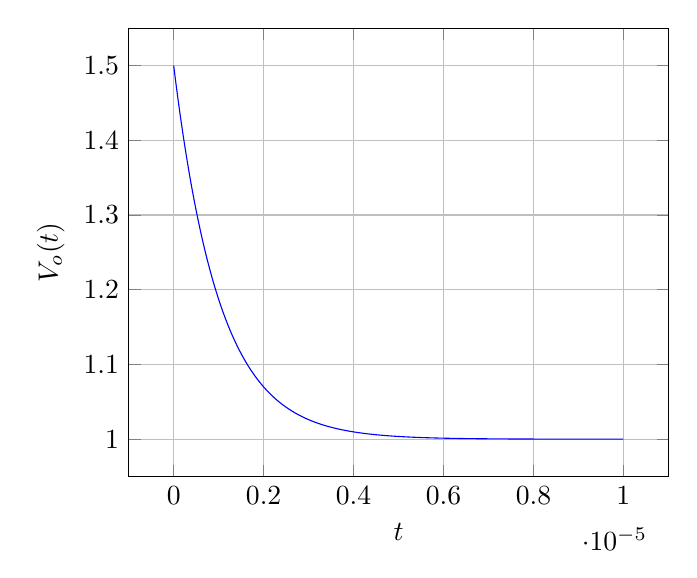
\begin{tikzpicture}
        \begin{axis}[enlargelimits=true,grid=major,ylabel=$V_o(t)$,xlabel=$t$]
            \addplot [blue,domain=0:0.00001,samples=200]{1+(1/2)*e^(-(10^6)*x)*cos(10^6*x)+(1/2)*e^(-10^6*x)*sin(10^6*x)};
        \end{axis}
    \end{tikzpicture}
\end{center}
\end{solution}




\end{document}
